\documentclass[12pt]{article}
\newif\ifanswer%\answertrue% comment out \answertrue to show/hide answers
\usepackage{../../preamble3}% preamble always after \newif\ifanswer
%\pagenumbering{gobble}
\title{MathCounts Competition Practice IV, January 2021 \\ Target Round}
\author{Patrick \& James Toche}
\date{Revised:~\today}

\begin{document}
\maketitle
\begin{minipage}{\textwidth}
\begin{abstract}\setlength{\parindent}{0pt}%
Notes on Target Round of MathCounts Competition Practice IV, January 2021. 
Questions are from MathCounts Foundation (\url{https://www.mathcounts.org/}). Copyright restrictions may apply. Written for personal use. 
Please report typos and errors over at \url{https://github.com/ptoche/Math/tree/master/mathcounts}. 
\end{abstract}
\end{minipage}

\thispagestyle{empty}
\clearpage

\section*{Target Round}


%%%%%%%%%%%%%%%%%%%%%%%%%%%%%%%%%%%%%%%%%%%%%%%%%%%%%%%%%%%%%%%%%%%%%%%%
\subsection*{1.}
Washington, D.C. has a land area of $68$ square miles and a population of $720,000$ people. What is the number of people per square mile in Washington, D.C.? Express your answer to the nearest hundred. 

\nopagebreak

\fbox{\phantom{ANSWER}}~people per square mile

\begin{answer}
\begin{align*}
\frac{720000\,\text{people}}{68\,\text{mi}^2}
  \approx 10588.24\,\text{people/mi$^2$}
\end{align*}
\begin{empheq}[box={\mathbox[colback=white]}]{equation*}
    10600 ~\text{people per square mile}
\end{empheq} 
\end{answer}
%%%%%%%%%%%%%%%%%%%%%%%%%%%%%%%%%%%%%%%%%%%%%%%%%%%%%%%%%%%%%%%%%%%%%%%%


%%%%%%%%%%%%%%%%%%%%%%%%%%%%%%%%%%%%%%%%%%%%%%%%%%%%%%%%%%%%%%%%%%%%%%%%
\subsection*{2.}
What is the maximum number of consecutive positive integers that can be added together before the sum exceeds $400$?

\nopagebreak

\fbox{\phantom{ANSWER}}

\begin{answer}
Minimize the sum of the first $n$ integers minus $400$:
\begin{align*}
\min_{n}\sum_{k=1}^{k=n}k-400 
  = \min_{n}\frac{n(n+1)}{2} 
\end{align*}
To get a quick order of magnitude, get an approximate solution to the associated quadratic equation:
\begin{align*}
n^2 + n - 800 
 & = \left(n + \frac{1}{2}\right)^2 - \left(\frac{1}{2}\right)^2 - 800 \\
 & = \left(n + \frac{1}{2}\right)^2 - \left(\frac{1}{2}\right)^2 - 784 - 6 \\
 & = \left(n + \frac{1}{2} - 28\right) \left(n + \frac{1}{2} + 28\right) - 6
\end{align*}
So the solution is less than $28$. We can check that $27$ gives:
\begin{align*}
\frac{27(27+1)}{2} = 27 \times 14 = 378
\end{align*}
The maximum number of consecutive positive integers is:
\begin{empheq}[box={\mathbox[colback=white]}]{equation*}
    27
\end{empheq} 
\end{answer}
%%%%%%%%%%%%%%%%%%%%%%%%%%%%%%%%%%%%%%%%%%%%%%%%%%%%%%%%%%%%%%%%%%%%%%%%


%%%%%%%%%%%%%%%%%%%%%%%%%%%%%%%%%%%%%%%%%%%%%%%%%%%%%%%%%%%%%%%%%%%%%%%%
\subsection*{3.}
Clifton left $280$ acres of land to be divided among his sons Al and Bob in the ratio $4{:}3$ respectively. How many acres should Al receive?

\nopagebreak

\fbox{\phantom{ANSWER}}~acres

\begin{answer}
Al would receive 
\begin{align*}
\frac{4}{4+3} \times 280 = 160
\end{align*}
\begin{empheq}[box={\mathbox[colback=white]}]{equation*}
    160~\text{acres}
\end{empheq} 
\end{answer}
%%%%%%%%%%%%%%%%%%%%%%%%%%%%%%%%%%%%%%%%%%%%%%%%%%%%%%%%%%%%%%%%%%%%%%%%


%%%%%%%%%%%%%%%%%%%%%%%%%%%%%%%%%%%%%%%%%%%%%%%%%%%%%%%%%%%%%%%%%%%%%%%%
\subsection*{4.}
George and Lea each toss a tetrahedral die with faces numbered $1$ through $4$, and then multiply the two resulting numbers. If the product is less than $9$, George wins; otherwise, Lea wins. What is the probability that Lea will win? Express your answer as a common fraction. 

\nopagebreak

\begin{minipage}[b]{\linewidth}
\fbox{\phantom{ANSWER}}\\
\mbox{---------------}\\
\fbox{\phantom{ANSWER}}
\end{minipage}

\begin{answer}
The product is less than $9$ if the faces show $(1,1)$, $(1,2)$, $(1,3)$, $(1,4)$, $(2,2)$, $(2,3)$, $(2,4)$. The number of ordered pairs is twice as many, or $14$, out of a total of $4^2=16$. The probability is therefore
\begin{align*}
\frac{14}{16} = \frac{7}{8}
\end{align*}
\begin{empheq}[box={\mathbox[colback=white]}]{equation*}
    \frac{7}{8}
\end{empheq} 
\end{answer}
%%%%%%%%%%%%%%%%%%%%%%%%%%%%%%%%%%%%%%%%%%%%%%%%%%%%%%%%%%%%%%%%%%%%%%%%

\iftoggle{showAnswers}{\newpage}

%%%%%%%%%%%%%%%%%%%%%%%%%%%%%%%%%%%%%%%%%%%%%%%%%%%%%%%%%%%%%%%%%%%%%%%%
\subsection*{5.}
How many rectangles of any size are in the diagram?

\begin{center}
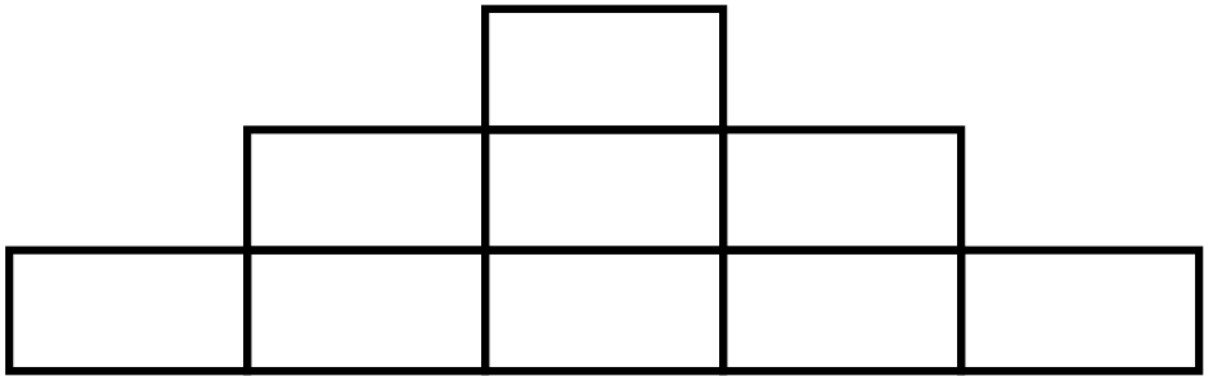
\includegraphics[height=3cm,page=1]{target-05-figure}
\end{center}

\nopagebreak

\fbox{\phantom{ANSWER}}~rectangles

\begin{answer}
There are $9$ rectangles of length $1$. There are $6$ rectangles of length $2$. There are $4$ rectangles of length $3$. There are $2$ rectangles of length $4$. There is $1$ rectangle of length $5$. There are $4$ rectangles of height $2$. There is $1$ rectangles of height $3$. There are $2$ rectangles of length $2$ and height $2$. There is $1$ rectangle of length $3$ and height $2$. 
\begin{align*}
9 + 6 + 2 + 1 + 4 + 1 + 2 + 1 = 26
\end{align*}
\begin{empheq}[box={\mathbox[colback=white]}]{equation*}
    26 ~\text{rectangles}
\end{empheq} 
\end{answer}
%%%%%%%%%%%%%%%%%%%%%%%%%%%%%%%%%%%%%%%%%%%%%%%%%%%%%%%%%%%%%%%%%%%%%%%%


%%%%%%%%%%%%%%%%%%%%%%%%%%%%%%%%%%%%%%%%%%%%%%%%%%%%%%%%%%%%%%%%%%%%%%%%
\subsection*{6.}
At the Word Store, each vowel sells for a different price, but all consonants are free. The word ``triangle'' sells for $\$6$, ``square'' sells for $\$9$, ``pentagon'' sells for $\$7$, ``cube'' sells for $\$7$ and ``tetrahedron'' sells for $\$8$. What is the cost of the word ``octahedron''? 

\nopagebreak

\$~\fbox{\phantom{ANSWER}}

\begin{answer}
Counting the vowels in each word and assigning the word's price yields the system:
\begin{align}
\label{eq:triangle}
1\,i + 1\,a + 1\,e & = 6 \quad\text{(triangle)} \\
\label{eq:square}
1\,u + 1\,a + 1\,e & = 9 \quad\text{(square)} \\
\label{eq:pentagon}
1\,o + 1\,a + 1\,e & = 7 \quad\text{(pentagon)} \\
\label{eq:cube}
       1\,u + 1\,e & = 7 \quad\text{(cube)} \\
\label{eq:tetrahedron}
1\,o + 1\,a + 2\,e & = 8 \quad\text{(tetrahedron)} \\
\label{eq:octahedron}
2\,o + 1\,a + 1\,e & = C \quad\text{(octahedron)} 
\end{align}
where $C$, the unknown, denotes the cost of ``octahedron''. 
Combining equation~(\ref{eq:pentagon}) with~(\ref{eq:octahedron}) yields $C = 1\,o + 7$. To find $C$, we now solve the system for $o$.  Subtracting~(\ref{eq:pentagon}) from (\ref{eq:tetrahedron}) gives $e=1$. Substituting into~(\ref{eq:cube}) gives $u=6$. Substituting into~(\ref{eq:square}) gives $a=7$. Finally substituting into~(\ref{eq:tetrahedron}) gives $o=-1$ (a negative price is a subsidy, a little unexpected). And thus $C=6$
\begin{empheq}[box={\mathbox[colback=white]}]{equation*}
    \$~ 6
\end{empheq} 
\end{answer}
%%%%%%%%%%%%%%%%%%%%%%%%%%%%%%%%%%%%%%%%%%%%%%%%%%%%%%%%%%%%%%%%%%%%%%%%


%%%%%%%%%%%%%%%%%%%%%%%%%%%%%%%%%%%%%%%%%%%%%%%%%%%%%%%%%%%%%%%%%%%%%%%%
\subsection*{7.}
All six faces of a large wooden cube are painted blue, and then the cube is divided into smaller unit cubes. If $486$ of the unit cubes have exactly one blue face, how many unit cubes make up the original large cube?

\nopagebreak

\fbox{\phantom{ANSWER}}~unit cubes

\begin{answer}
Take a cube made up of $n^3$ cubelets. The cubelets with exactly one painted side are found on the surface, excluding edges and corners. Each of the six faces has $(n-2)^2$ ``inner'' cubelets. Now solve for $n$:
\begin{align*}
6(n-2)^2 & = 486 \\
(n-2)^2 & = 81 \\
(n-2) & = \pm 9
\end{align*}
The solution is the positive root, so $n=9+2=11$ and the total number of cubelets $11^3=1331$
\begin{empheq}[box={\mathbox[colback=white]}]{equation*}
    1331 ~\text{unit cubes}
\end{empheq} 
\end{answer}
%%%%%%%%%%%%%%%%%%%%%%%%%%%%%%%%%%%%%%%%%%%%%%%%%%%%%%%%%%%%%%%%%%%%%%%%


%%%%%%%%%%%%%%%%%%%%%%%%%%%%%%%%%%%%%%%%%%%%%%%%%%%%%%%%%%%%%%%%%%%%%%%%
\subsection*{8.}
Darla can complete a job in $8$ hours, while Lonnie can complete the same job in $6$ hours. Both Darla and Lonnie begin working on the job together. After working together for $3$ hours, how much of the job is left to be completed? Express your answer as a common fraction. 

\nopagebreak

\begin{minipage}[b]{\linewidth}
\fbox{\phantom{ANSWER}}\\
\mbox{---------------}\\
\fbox{\phantom{ANSWER}}
\end{minipage}


\begin{answer}
First note that if two Lonnies worked for $3$ hours, that would be equivalent to Lonnie working $6$ hours and completing exactly one job. Since Darla is less productive than Lonnie, it follows that together they will complete (a little) less than one job. 
Let $h$ denote hours and $p$ productivity so that $ph$ denotes the output. Darla produces one unit of output (a ``job'') in $8$ hours, so her productivity is $1/8$th of a job per hour. Likewise Lonnie has productivity $1/6$ (Lonnie's productivity is greater than Darla's).
Together, Darla and Lonnie work for $h=3$ hours and produce:
\begin{align*}
  3 \times \frac{1}{8} +3 \times \frac{1}{6} 
    = 3 \times \frac{3+4}{3 \times 8} 
    = \frac{7}{8}
\end{align*}
which is indeed a little less than $1$ job.
\begin{empheq}[box={\mathbox[colback=white]}]{equation*}
    \frac{7}{8}
\end{empheq} 
\end{answer}
%%%%%%%%%%%%%%%%%%%%%%%%%%%%%%%%%%%%%%%%%%%%%%%%%%%%%%%%%%%%%%%%%%%%%%%%


\end{document}